\subsection{Bisimilarity
of pOCA is in PSPACE}\label{sec:bispOCAinPSPACE}

The bisimilarity problem for (non-probabilistic)
one-counter automata is  PSPACE-complete, as shown
in~\cite{BGJ:Concur10}. It turns out that for pOCA we get
PSPACE-completeness as well.
The lower bound is shown in Section~\ref{sec-lower-bounds}; here
we show:

\begin{theorem} \label{thm-bisim-pOCA-inPspace}
The bisimilarity problem for pOCA is in PSPACE, even
if we present the instance
 ,
 (for which we ask if )
by a shorthand using  written in binary.
\end{theorem}
The reduction underlying
Theorem~\ref{thm:prob-to-nondet} would only provide an
exponential-space upper bound, so
we give a pOCA-specific polynomial-space algorithm.
In fact, we adapt the algorithm from~\cite{BGJ:Concur10};
the principles are the same but some
ingredients have to be slightly modified.
The following text is meant to give the idea in a self-contained
manner, though at a more abstract
level than in~\cite{BGJ:Concur10}.
The main difference is in the notion of local consistency, discussed
around Proposition~\ref{prop:localconsistency}.

Similarly as~\cite{BGJ:Concur10},
we use a geometrical presentation of relations on
the set of configurations (Fig.~\ref{fig:belts} reflects such a
presentation).
A relation can be identified with
a / (or YES/NO)
colouring of the ``grid''  :


\begin{figure}[t]
\subfigure[Partition of a grid, and a moving vertical window~of~width~3\label{fig:belts}]{
\begin{tikzpicture}[x = {(1.9cm,0cm)}, y = {(0cm,1.9cm)}, z = {(-0.5cm,0.6cm)},font=\scriptsize]
\path [name path=w1](2.0,0,0)--(2.0,3,0);
 \path [name path=w2](2.0,0,1)--(2.0,3,1);
 \path [name path=ww1](2.2,0,0)--(2.2,3,0);
 \path [name path=ww2](2.2,0,1)--(2.2,3,1);
 \path [name path=www1](2.4,0,0)--(2.4,3,0);
 \path [name path=www2](2.4,0,1)--(2.4,3,1);
 \path [name path=r1](1,0.3,0) -- (3,0.8,0);
 \path [name path=r2](1,0.3,1) -- (3,0.8,1);
 \path [name path=u1](0.9,1,0) -- (2.9,3,0);
 \path [name path=u2](0.9,1,1) -- (2.9,3,1);
 \path [name intersections={of= w1 and r1, name=A}];
 \path [name intersections={of= w2 and r2, name=B}];
 \path [name intersections={of= w1 and u1, name=C}];
 \path [name intersections={of= w2 and u2, name=D}];
 \path [name intersections={of= ww1 and r1, name=Aw}];
 \path [name intersections={of= ww2 and r2, name=Bw}];
 \path [name intersections={of= ww1 and u1, name=Cw}];
 \path [name intersections={of= ww2 and u2, name=Dw}];
 \path [name intersections={of= www1 and r1, name=Aww}];
 \path [name intersections={of= www2 and r2, name=Bww}];
 \path [name intersections={of= www1 and u1, name=Cww}];
 \path [name intersections={of= www2 and u2, name=Dww}];

\draw[-latex'] (0,0,1) -- (3,0,1);

\draw[path fading=north] (1,0.1,1) -- (3,0.6,1);
 \draw[path fading=north] (1,0.3,1) -- (3,0.8,1);
 \shade[opacity=0.6, shading angle=90] (1,0.1,1) -- (1,0.3,1) -- (3,0.8,1) -- (3,0.6,1) -- cycle;
 \shade[opacity=0.6, shading angle=120] (1,0.1,0) -- (3,0.6,0) -- (3,0.6,1) -- (1,0.1,1) -- cycle;

\draw[path fading=east] (0.9,1,1) -- (2.9,3,1);
 \draw[path fading=east] (1,0.9,1) -- (3,2.9,1);
 \shade[opacity=0.6, shading angle=125] (0.9,1,1) -- (1,0.9,1) -- (3,2.9,1) -- (2.9,3,1) -- cycle;
 \shade[opacity=0.6, shading angle=145] (1,0.9,0) -- (3,2.9,0) -- (3,2.9,1) -- (1,0.9,1) -- cycle;

\path[fill=gray,opacity=0.7] (0,1,0) rectangle (1,0,0);
 \path[fill=gray,opacity=0.7] (0,1,1) rectangle (1,0,1);
 \path[fill=gray,opacity=0.7] (1,1,1) -- (1,1,0) -- (1,0,0) -- (1,0,1) -- cycle;
 \path[fill=gray,opacity=0.7] (0,1,1) -- (0,1,0) -- (0,0,0) -- (0,0,1) -- cycle;
 \node at (0.4,0.5,0) {\parbox{1.5cm}{\centering initial \\ space}};

\draw[path fading=north] (0.2,1,0) -- (0.5,3,0);
 \draw[path fading=north] (0.2,1,1) -- (0.5,3,1);
 \draw[path fading=north] (0.5,1,0) -- (0.8,3,0);
 \draw[path fading=north] (0.5,1,1) -- (0.8,3,1);
 \shade[opacity=0.6, shading angle=160] (0.2,1,0) -- (0.5,3,0) -- (0.5,3,1) -- (0.2,1,1) -- cycle;
 \shade[opacity=0.6, shading angle=180] (0.2,1,0) -- (0.5,1,0) -- (0.8,3,0) -- (0.5,3,0) -- cycle;
 \shade[opacity=0.6, shading angle=160] (0.5,1,0) -- (0.8,3,0) -- (0.8,3,1) -- (0.5,1,1) -- cycle;
 \shade[opacity=0.6, shading angle=180] (0.2,1,1) -- (0.5,1,1) -- (0.8,3,1) -- (0.5,3,1) -- cycle;
 \node[rotate=80] at (0.4,1.5,0) {belt space};

\path[opacity=0.6,fill] (2.4,0,0) -- (Aww-1) -- (Bww-1) -- (2.4,0,1) -- cycle;
 \path[opacity=0.6,fill] (2.2,0,0) -- (Aw-1) -- (Bw-1) -- (2.2,0,1) -- cycle;
 \path[opacity=0.6,fill] (2,0,0) -- (A-1) -- (B-1) -- (2,0,1) -- cycle;

\draw[path fading=north] (1,0.1,0) -- (3,0.6,0);
 \draw[path fading=north] (1,0.3,0) -- (3,0.8,0);
 \shade[opacity=0.6, shading angle=120] (1,0.3,0) -- (3,0.8,0) -- (3,0.8,1) -- (1,0.3,1) -- cycle;
\path[opacity=0.6,fill] (Aww-1) -- (Cww-1) -- (Dww-1) -- (Bww-1) -- cycle;
 \path[opacity=0.6,fill] (Aw-1) -- (Cw-1) -- (Dw-1) -- (Bw-1) -- cycle;
 \path[opacity=0.6,fill] (A-1) -- (C-1) -- (D-1) -- (B-1) -- cycle;
 \shade[opacity=0.6, shading angle=90] (1,0.1,0) -- (1,0.3,0) -- (3,0.8,0) -- (3,0.6,0) -- cycle;
 \node[rotate=14] at (1.4,0.32,0) {belt space};

\draw[path fading=east] (0.9,1,0) -- (2.9,3,0);
 \draw[path fading=east] (1,0.9,0) -- (3,2.9,0);
 \shade[opacity=0.6, shading angle=145] (0.9,1,0) -- (2.9,3,0) -- (2.9,3,1) -- (0.9,1,1) -- cycle;
\path[opacity=0.6,fill] (2.4,3,0) -- (Cww-1) -- (Dww-1) -- (2.4,3,1) -- cycle;
 \path[opacity=0.6,fill] (2.2,3,0) -- (Cw-1) -- (Dw-1) -- (2.2,3,1) -- cycle;
 \path[opacity=0.6,fill] (2,3,0) -- (C-1) -- (D-1) -- (2,3,1) -- cycle;
 \shade[opacity=0.6, shading angle=145] (0.9,1,0) -- (1,0.9,0) -- (3,2.9,0) -- (2.9,3,0) -- cycle;
 \node[rotate=45] at (1.3,1.3,0) {belt space};


\draw[-latex'] (0,0,1) -- (0,3,1) node[pos=0.9,left] {};
 \draw[-latex'] (0,0,0) -- (3,0,0) node[pos=1,right] {};
 \draw[-latex'] (0,0,0) -- (0,3,0);
 \draw (0,0,0) -- (0,0,1) node[pos=0.0,left] {}
  node[pos=0.35,left] {}
  node[pos=0.65,left] {}
  node[pos=1,left] {};
\node[rotate=70] at (0.9,2,0) {background space};
 \node[rotate=35] at (1.45,1,0) {\parbox{1.5cm}{\centering background\\ space}};
\draw (2,0,0) -- (2,3,0);
 \draw (2.2,0,0) -- (2.2,3,0);
 \draw (2.4,0,0) -- (2.4,3,0);
\end{tikzpicture}
 }
\subfigure[AND-gadget (top) and OR-gadget (bottom)\label{fig:gadgets}]{
\parbox[b]{3.8cm}{
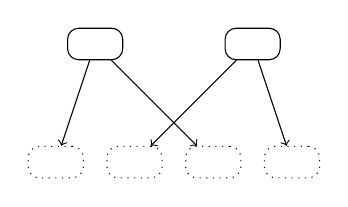
\begin{tikzpicture}[font=\scriptsize]
\tikzstyle{every node} = [inner sep=2pt];
\tikzstyle{mystate} = [minimum height=4mm, minimum width=7mm,rounded corners];



\node (aa) at (0.5,1.5) [mystate,draw] {};
\node (bb) at (2.5,1.5) [mystate,draw] {};
\node (cc) at (0,0) [mystate,draw,dotted] {};
\node (dd) at (1,0) [mystate,draw,dotted] {};
\node (ee) at (2,0) [mystate,draw,dotted] {};
\node (ff) at (3,0) [mystate,draw,dotted] {};

\draw[->] (aa)--(cc);
\draw[->] (bb)--(dd);
\draw[->] (aa)--(ee);
\draw[->] (bb)--(ff);
\end{tikzpicture}

 
\bigskip
\noindent
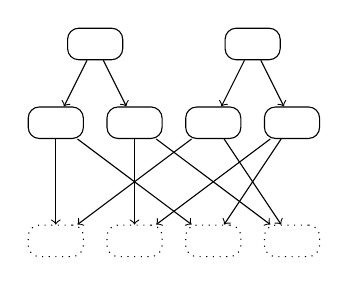
\begin{tikzpicture}[font=\footnotesize]
\tikzstyle{every node} = [inner sep=2pt];
\tikzstyle{mystate} = [minimum height=4mm, minimum width=7mm,rounded corners];


\node (a)  at (0.5,3) [mystate,draw] {};
\node (b) at (2.5,3) [mystate,draw] {};
\node (c) at  (0,2) [mystate,draw] {};
\node (d) at  (1,2) [mystate,draw] {};
\node (e) at  (2,2) [mystate,draw] {};
\node (f) at  (3,2) [mystate,draw] {};
\node (g) at  (0,0.5) [mystate,draw,dotted] {};
\node (h) at  (1,0.5) [mystate,draw,dotted] {};
\node (i) at  (2,0.5) [mystate,draw,dotted] {};
\node (j) at  (3,0.5) [mystate,draw,dotted] {};
\draw[->]  (a) -- (c);
\draw[->]  (a) -- (d);
\draw[->]  (b) -- (e);
\draw[->]  (b) -- (f);
\draw[->]  (c) -- (g);
\draw[->]  (d) -- (h);
\draw[->]  (e) -- (j);
\draw[->]  (f) -- (i);
\draw[->]  (e) -- (g);
\draw[->]  (f) -- (h);
\draw[->]  (c) -- (i);
\draw[->]  (d) -- (j);
\end{tikzpicture}

 }}
\caption{Figures for Section \ref{sec:bispOCAinPSPACE} (left) and \ref{sec-lower-bounds} (right)}
\end{figure}


\begin{definition}
For a
relation  on ,
by the  \emph{(characteristic) colouring}  we mean
the function

where  if and only if .
Given (a colouring)
, by
 we denote the relation
.
\end{definition}
The algorithm uses the fact that  is ``regular'', i.e.
 is a (special) semilinear set.
More concretely, there are polynomials 
(independent of the pOCA~) such that the following partition of the grid

(sketched in Fig.~\ref{fig:belts})
has an important property specified later.
If , hence , then the grid is
partitioned into three parts: the \emph{initial-space}, i.e.
, the \emph{belt-space},
which is given by at most  linear belts, with the slopes  where
 and with the (vertical) thickness bounded by
, and the rest, called the \emph{background}.
Moreover,  is sufficiently large w.r.t. , so that
 the belts are separated by the background
 outside
the initial space.

The mentioned important property is that
there is a period , given by an exponential function of ,
such that
if two points  and 
(for )
are both in the background, for both  larger then a polynomial bound, then
 has the same value for both these points; in other words,
 colours the background periodically.
Another important ingredient is the locality of the bisimulation conditions,
resulting from the fact that the counter value can change by at most 
per step.

To explain the ``grid-partition'', we start with
 considering the finite automaton 
underlying ;
 behaves like  ``pretending'' that the
counter is always positive.





\begin{definition}\label{D underlying}
For a pOCA
,
in the {\em underlying finite pLTS}
 we have
a transition  if and only if there is a transition 
such that  (for all
).
\end{definition}
Using standard partition-refinement arguments, we observe
that  on  when .
For configurations of~ we now define the distance
 to the set of configurations which are
``INCompatible'' with .
\begin{definition}
Assuming a pOCA
, where ,
\\
we define  and
 as follows:
\begin{itemize}
\item
 (where 
is a state in ),
\item
\,;
we set .
\end{itemize}
\end{definition}
Since  (by induction on ), and thus
 implies
,
we can surely construct  for a given pOCA in polynomial space.


\begin{proposition}
\label{L nonreachable}
\hfill
\begin{enumerate}
\item
If  then .
\item
\mbox{If 
then
 iff .}
\end{enumerate}
\end{proposition}
The proof is the same as in the non-probabilistic case.
(Point 1 is obvious. For Point 2 we verify that the set

is a bisimulation.)

Consider a shortest path from  to  (for large ).
It is not hard to prove (as in~\cite[Lemma 10]{BGJ:Concur10}) that such a path can be based on iterating
a simple counter-decreasing cycle (of length
), possibly preceded by a polynomial prefix and followed by a
polynomial suffix.
So (finite)  can be always expressed
by the use of linear functions  where
 are the length and the decreasing effect of a simple
cycle and  is bounded by a polynomial in .
It follows that if we have ,
then ,
which shows that
 lies in one of the above mentioned belts, or in the
initial space when  are small.



As a consequence, in the background points 
we have either ,
and  if and only if ,
or 
(and thus  ).
So we can easily compute  for any background point in
polynomial space.

The above mentioned shortest paths to  also show that
if we choose  (so ) then
we have
 if and only if  (for  larger than
some polynomial bound), since the counter-effect of each simple cycle
divides .
Hence
 is a background period as mentioned above.

A nondeterministic algorithm, verifying that  for   in the initial or belt-space,
is based on ``moving a
vertical window of width '' (as depicted in Fig.~\ref{fig:belts});
in each phase, the window is moved by  (to the right),
its intersection with the initial and belt space
(containing polynomially many
points) is computed, a colouring
on this intersection is guessed
 ( is intended)
and its (local) consistency is
checked (for which also 
on the neighbouring background points is computed).
More precisely, in the first, i.e. leftmost, window position a
colouring in all
three (vertical) slices is guessed and the local consistency in the first two
slices is checked; after any later shift of the window
by one to the right, a colouring in
the new (the rightmost) slice is
guessed (the guesses in the previous two slices being remembered), and
the consistency in the current middle slice is checked.
If this is successfully performed
for exponentially many steps,
after  has been coloured with , then
it is guaranteed that
the algorithm could successfully run forever; the pigeonhole principle
induces that each belt could be periodically coloured, with an
exponential period compatible with the period of the background-border
of the belt.
Such a successful run of the algorithm, exponential in time but
obviously only
polynomial in the required space, is thus a witness of . Since PSPACE=NPSPACE, we have thus sketched a proof
 of Theorem~\ref{thm-bisim-pOCA-inPspace}.




It remains to define precisely the consistency of a colouring,
guaranteeing that a successful run of the algorithm really witnesses
. (As already mentioned, this is the main
change wrt~\cite{BGJ:Concur10}.)
We use the following particular variant of
characterizing (probabilistic) bisimilarity.
Given a pLTS
,
we say that  is \emph{consistent w.r.t.}
a relation  on  (not necessarily an equivalence)
if
for each  there is  ,
and conversely for each  there is  ,
such that  are -equivalent where

is the least equivalence containing the set
.
A \emph{relation}  is \emph{consistent} if each  is consistent w.r.t.
. The following proposition can be verified along the standard
lines.


\begin{proposition}\label{prop:localconsistency}
 is consistent.
If  is consistent then .
\end{proposition}
Our algorithm can surely (locally) check the above defined
consistency of the
constructed 
(i.e. of ).


